% !TEX root = ../main.tex
\chapter{Model creation} \label{ch:model}
% TITOLO DA VALUTARE

This chapter will outline the approach suggested by IBM Reserch for tackling the challange introduced in \textbf{\nameref{ch:introduction}} regarding fault detection and diagnosis (FDD). %TODO

\section{State of the art}
Nowadays, as extensively analyzed by \textcite{methods_for_diagnostic}, FDD approaches fall in either one of the following three categories: physycal model based approaches, data driven approaches and rule-based approaches. The rationales behind these approaches are detailed in \autoref{subsec:phy_models}, \autoref{subsec:data_models} and in \autoref{subsec:rule_models}. Still, each of these approaches share common limitations that can be summarized as
\begin{itemize}
  \item they can be applied to a single, specific building
  \item they requires large manual effort and expertise
  \item deploy can take several weeks
  \item they neglect strong interactions between systems
\end{itemize}

\subsection{Physycal model approach} \label{subsec:phy_models}
These approaches require a physycal model (e.g ordinary differential equations) of the building and its components. They are highly precise in diagnosing faults given a correct model, however, deriving the models is no trivial task and requires times and expertise. On top of this, derived models are building, system and location specific and are difficult to adapt to other buildings than the one they are thought for even if they share similar structure and similar components, thus limiting the scalability of this approach.

\subsection{Data driven approach} \label{subsec:data_models}
Data driven approaches completely rely on building's sensor data. They assume that access to a large dataset of hystorical data is granted. There's little to no need for any \textit{a priori} knowledge of the processes involved. Black-box data driven approaches derive the model in the form of a input-output relationship which parameters aren't correlated with the actual physical parameter (e.g artificial neural networks, regression) while grey-box data driven approaches take advantage of simplified physical relationships between measured quantities (e.g principal component analysys) and rely on statistical methods for estimating their parameters. Even though these methods don't suffer from scalability issues they are limited to fault detection and lack in diagnosis capabilities.

\subsection{Rule-based approach} \label{subsec:rule_models}
The rule-based approach is the most common in traditional FDD applications. It uses domain knowledge and expertise in order to derive a series of simple \textit{if-then-else} rules or some kind of decision trees along with a series of thresholds and confidence intervals; during system operations data are evaluated against this rules and countermeasures are eventually taken. Even though this is the most common approach, it still needs a lot of manual effort and requires access to domain knowledge so these requirements still limit portability and scalability of applications based on this technique.

\section{IBM Research approach}
The approach developed by IBM Research is based on a combination of the three aformentioned concepts to overcome their disadvantages. It models high level physical processes in the systems to derive diagnosis rules, it parametrize the rules using data analytics techniques and applies them during systmes operations. The strength of the semantic approach lies in its capability to automatically infer knowledge given a building, its sensors and their data. This lead to a semi-automated process that limit the manual effort needed as shown in \autoref{fig:approach_overview}.
\begin{figure}
  \centering
  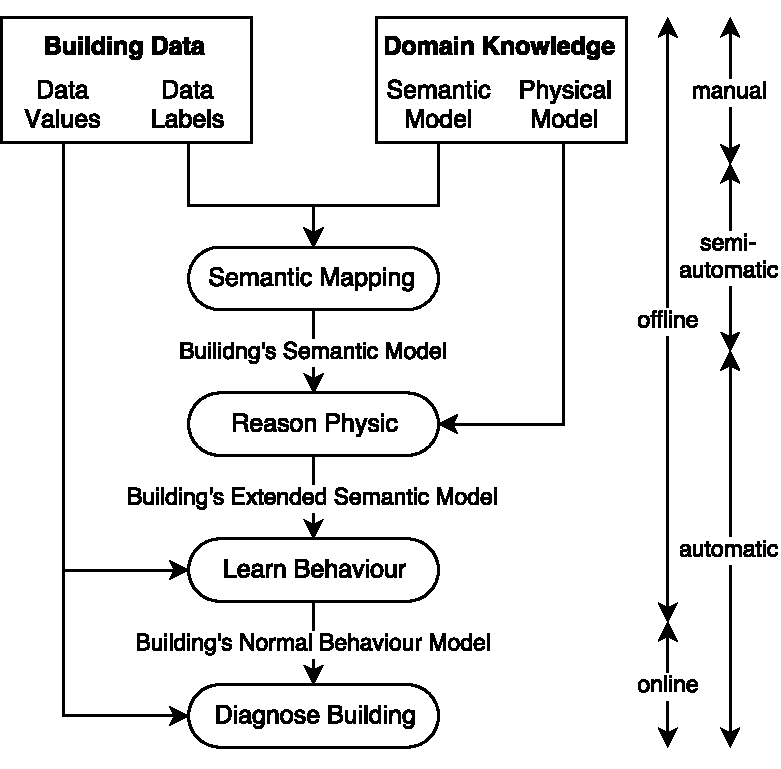
\includegraphics[width=0.7\textwidth]{approach_overview.pdf}
  \caption{IBM Reserch approach, overview}
  \label{fig:approach_overview}
\end{figure}

The proposed approach needs 3 inputs to produce the diagnosis of a given anomaly
\begin{itemize}
  \item building data: assumed available in the building's Building Management System (BMS)
  \item semantic model: specified through the use of concepts from domain ontologies Brick (\autoref{subsec:brick}) e SSNO (\autoref{subsec:ssn})
  \item physycal model: the model of the physical dependencies between subsystems of the building. The physical processes are modelled through concepts presented in the extended SSNO (\autoref{ssubsec:extended_ssno})
\end{itemize}
these inputs are processed through the various stages to produce the complete model of the building and its internal processes. Details about the different phases are given in the following pages.

\subsection{Semantic Mapping}
Building a semantic model for a specific building needs knowledge on the type of sensors, meters and various equipment available in said building, their location and their semantic meaning in the chosen ontologies. These informations are usually stored in BMS through labels that, despite some kind of standardization efforts, are usually vendor specific; in some cases even the same vendor ends up changing its labeling schemes throughout the years. Even though there is no common ground to evaluate these labels, usually they are comprised of a series of abbreviations, eventually separated by some special character (e.g ``\textunderscore''), that gives informations about the device's ID, function and location (or the equipment it is part of). An air temperature sensor in a room on ground floor can be labeled AIR\textunderscore TEMP\textunderscore R3GF while another air temperature sensor in a room on the first floor may ends up being labeled as RATSF1R9; both the sensors represent a common semantic resource in an ontology and need to be mapped that concept. This process is called semantic mapping. Existing approaches are differentiated in three different types \cite{semantic_mapping}
\begin{itemize}
  \item semi-automatic: they offer a tool assisting the user in labelling the point to corresponding semantic types and are based on advanced text mining techniques (e.g regular expressions, classifiers)
  \item data driven: these approaches try to recover the meta-data given the timeseries. It is based on the concept that different data-points exhibiting similar timeseries behaviour should be similar themselves.
  \item active feedback: in these kind of approaches a series of known events are injected into the system and datapoints semantic model is derived observing the effect of the event injection.
\end{itemize}

\subsubsection{Building Energy Asset Discovery tool}
BEAD \cite{bead} is the tool developed by IBM Research for assisting user in the process of discovery and tagging of sensors. The tool is based on dictionaries of the type $\mathcal{D}:\mathcal{A}\rightarrow \mathcal{MS}$ where $\mathcal{A}$ is the set of all relevant acronyms and $\mathcal{MS}$ is the set of markerset; each markerset is a set of markers, or keywords. These concepts are closely related to those of tagset and tag found in the Brick ontology and this duality allows the association of the sensor with the correct semantic type as described by Brick (see \ref{subsec:brick}). The dictionary contains the most common acronyms found in BMS and it is further extended by the markers (tags) from the Brick ontology, such that a tag maps to itself, e.g Temperature$\rightarrow$\{Temperature\}. The tool take a label from the BMS and compute a similarity score against the dictionary entries and guide the user in the labeling process. For example, given the following dictionary
\begin{description}[noitemsep]
  \item \textbf{d1}: RAT$\rightarrow$\{Return, Air, Temperature\}
  \item \textbf{d2}: RAT$\rightarrow$\{Room, Air, Temperature\}
  \item \textbf{d3}: SAT$\rightarrow$\{Supply, Air, Temperature\}
  \item \textbf{d4}: OAT$\rightarrow$\{Outdoor, Air, Temperature\}
  \item \textbf{d5}: Temp$\rightarrow$\{Temperature\}
  \item \textbf{d6}: Temperature$\rightarrow$\{Temperature\}
\end{description}
the label RATSF1R9 (Room Air Temperature Sensor, Floor 1, Room 9) has a high similarity with both RAT$\rightarrow$\{Return, Air, Temperature\} and RAT$\rightarrow$\{Room, Air, Temperature\}, so it's up to the user to understand the meaning and choose the right markerset. In a similar fashion it is possible to extract information on the location of a sensor or the asset it is related to, as shown in \autoref{tab:bead_dictionary}.
\begin{table}
  \centering
  \caption{Dictionary extended with assets' informations}
  \label{tab:bead_dictionary}
  \begin{tabular}{lll}
    \hline
    \textbf{Label} & \textbf{Asset} & \textbf{Marketset}                       \\\cline{1-3}
    U6\textunderscore RAT        & AHU6  & \{Return, Air, Temperature\}    \\
    U6\textunderscore DAT        & AHU6  & \{Discharge, Air, Temperature\} \\
    AHU7\textunderscore RAT      & AHU7  & \{Return, Air, Temperature\}    \\
    AHU7\textunderscore SAT      & AHU7  & \{Supply, Air, Temperature\}    \\
    AU9\textunderscore RET\textunderscore TEMP & AHU9  & \{Return, Air, Temperature\}    \\
    AU9\textunderscore SUP\textunderscore TEMP & AHU9  & \{Supply, Air, Temperature\}
  \end{tabular}
\end{table}

this process clearly requires human supervision, hence the definition of semi-automatic, but through this approach the operator has to manually inspect a smaller subset of all the possible marketsets \cite{semantic_mapping} thus taking minutes instead of several weeks to complete the semantic mapping. The output of this process is the semantic model of the specific building according to the chosen ontology. A chart illustrating the whole process is shown in \autoref{fig:semantic_mapping}.

\begin{figure}
  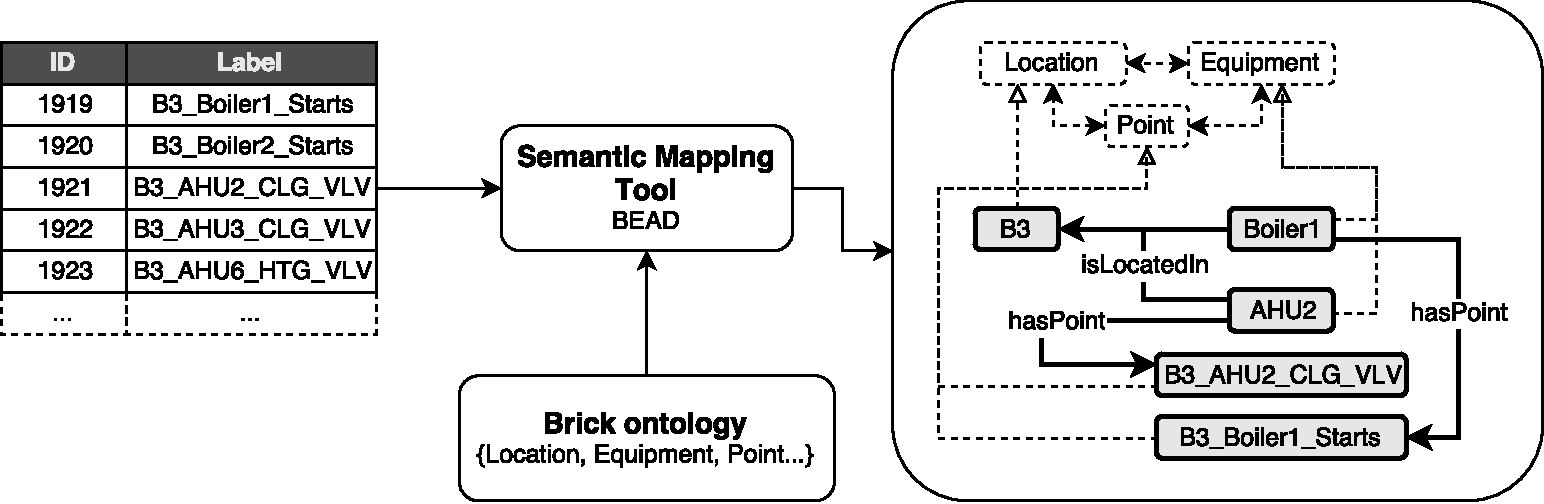
\includegraphics[width=1\textwidth]{semantic_mapping.pdf}
  \caption{Semantic mapping process}
  \label{fig:semantic_mapping}
\end{figure}
